\begin{savequote}[75mm] 
Nguyễn Đức Mạnh
\end{savequote}

\chapter{Giải pháp đề xuất}

\section{Tổng Quan Kiến Trúc Hệ Thống}

Hệ thống nhận dạng phiếu trắc nghiệm được thiết kế để xử lý ảnh đầu vào và trích xuất tự động thông tin định danh. Quá trình xử lý bao gồm các bước: chuyển đổi ảnh sang grayscale, làm mờ bằng Gaussian để giảm nhiễu, phát hiện cạnh bằng thuật toán Canny, và sử dụng Hough Transform để xác định các đoạn thẳng. Dựa trên các đoạn thẳng này, hệ thống xác định vị trí bảng metadata, chia thành lưới các ô tương ứng với chữ số, và đánh giá mức độ tô đậm của từng ô để nhận diện kết quả.

Toàn bộ kiến trúc hệ thống tuân theo quy trình xử lý từ tiền xử lý ảnh đến phân tích mức độ tô, đảm bảo độ chính xác cao và khả năng xử lý hàng loạt phiếu trắc nghiệm trong thời gian ngắn.

\section{Phân Tích Thách Thức và Yêu Cầu}

Trong thực tế, hệ thống phải xử lý nhiều loại ảnh khác nhau, không phải lúc nào cũng đạt chất lượng lý tưởng. Các ảnh bị mờ, lệch hoặc có ánh sáng không đều sẽ gây khó khăn cho quá trình phát hiện cạnh và xác định vùng bảng.

Ngoài ra, nếu các đường kẻ trong bảng không liền mạch, việc phân chia lưới ô có thể bị sai lệch, ảnh hưởng đến kết quả nhận dạng. Do đó, hệ thống cần có khả năng làm sạch ảnh hiệu quả, kết hợp với các kỹ thuật phát hiện hình học đủ mạnh để xử lý trong môi trường thực tế.

Yêu cầu cốt lõi là đảm bảo độ chính xác nhận dạng ký tự cao, đồng thời tối ưu hóa thời gian xử lý để phù hợp với các ứng dụng quy mô lớn.

\section{Chuẩn bị dữ liệu}







\section{Phát Hiện Vùng Metadata}

Để phát hiện vùng chứa thông tin định danh, hệ thống thực hiện các bước sau:

Đầu tiên, ảnh đầu vào được chuyển sang dạng grayscale và làm mờ để loại bỏ nhiễu. Sau đó, thuật toán Canny được sử dụng để phát hiện các cạnh rõ nét. Hệ thống áp dụng phát hiện contour để tìm vùng có diện tích lớn nhất — là vùng chứa bảng metadata.

Hough Transform tiếp tục được dùng để phát hiện các đường thẳng trong ảnh, từ đó phân loại thành các đường ngang và dọc. Một hàm hợp nhất các đoạn thẳng được sử dụng để gom nhóm các đường gần nhau, giúp xác định biên bảng một cách chính xác và ổn định.

\begin{figure}[h]
    \centering
    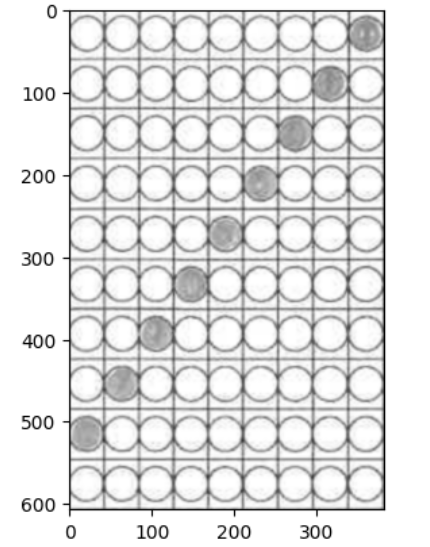
\includegraphics[width=0.5\linewidth]{figures/a1.png}
    \caption{Ảnh sau khi cắt vùng bảng metadata}
    \label{fig:enter-label}
\end{figure}

\section{Trích Xuất Thông Tin Định Danh}

Sau khi vùng chứa bảng metadata được xác định, hệ thống tiến hành trích xuất thông tin định danh như mã số sinh viên hoặc mã đề thi bằng cách chia khu vực này thành một lưới gồm nhiều ô nhỏ. Mỗi cột ứng với một chữ số, còn mỗi hàng đại diện cho giá trị từ 0 đến 9.

\subsection*{Cắt bảng và chia lưới}

Ảnh đầu vào được cắt chính xác để giữ lại vùng chứa bảng định danh bằng hàm \texttt{adaptive\_grid\_crop}. Vùng bảng được chia thành lưới $10 \times N$, với $N$ là số lượng chữ số cần nhận dạng. Mỗi ô nhỏ trong lưới là một vùng ảnh riêng biệt.

\subsection*{Tạo vùng mặt nạ hình tròn}

Mỗi ô chứa một hình tròn – vùng mà thí sinh sẽ tô để chọn số. Thay vì xử lý toàn bộ ô, hệ thống chỉ phân tích các pixel nằm trong mặt nạ hình tròn được tạo tự động tại tâm của ô.

\begin{itemize}
    \item \textbf{Tâm hình tròn} được xác định tại trung điểm của ô: $(w/2, h/2)$ với $w$ và $h$ là chiều rộng và chiều cao của ô.
    \item \textbf{Bán kính hình tròn} được đặt là $0.45 \cdot \min(w, h)$, đảm bảo vùng phân tích nằm gọn trong vòng tròn.
    \item \textbf{Mặt nạ (mask)} là một ma trận nhị phân có giá trị 1 bên trong vòng tròn và 0 bên ngoài.
\end{itemize}

Việc sử dụng mặt nạ hình tròn giúp hệ thống chỉ tập trung vào phần được yêu cầu tô, loại bỏ nhiễu từ viền hoặc phần trắng xung quanh.

\subsection*{Phân tích mức độ tô}

Hệ thống áp dụng hai phương pháp để tính toán mức độ tô bên trong hình tròn:

\vspace{0.5em}
\noindent
\textbf{1. Adaptive Threshold:}  
Ảnh được chuyển thành nhị phân bằng ngưỡng thích nghi. Sau đó, hệ thống tính tỷ lệ pixel đen nằm trong mặt nạ tròn. Giá trị này phản ánh trực tiếp mức độ tô.

\vspace{0.5em}
\noindent
\textbf{2. Trung bình mức xám:}  
Tính trung bình cường độ pixel trong vùng hình tròn. Mức tô được chuẩn hóa về khoảng [0, 1], trong đó 0 là sáng nhất (không tô), 1 là tối nhất (tô đậm).

\subsection*{Xác định chữ số tô}

Đối với mỗi cột, hệ thống sắp xếp các ô theo mức độ tô giảm dần. Kết quả được xác định theo các ngưỡng được thiết lập như sau:

\begin{itemize}
    \item Nếu hai ô có mức tô cao và chênh lệch nhỏ: đánh dấu là \texttt{M} (nhiều ô được tô).
    \item Nếu chỉ một ô vượt ngưỡng rõ rệt: nhận dạng là chữ số tương ứng.
    \item Nếu không ô nào thỏa điều kiện: gán là \texttt{X} (không xác định).
\end{itemize}

Mặc định, hệ thống sử dụng ngưỡng tô tối thiểu là $0.25$ và độ chênh lệch $0.15$ để phân biệt giữa các trường hợp.

\subsection*{Lưu kết quả và trực quan hóa}

Thông tin từng ô (tọa độ, tỷ lệ tô, trạng thái nhận dạng) được lưu vào tệp \texttt{.csv}, hỗ trợ việc phân tích sau này. Đồng thời, hệ thống tạo ảnh trực quan hoá kết quả, trong đó:

\begin{itemize}
    \item Màu xanh lá: ô được nhận dạng rõ ràng.
    \item Màu đỏ: ô không xác định.
    \item Màu vàng: có nhiều ô cùng mức tô.
\end{itemize}

Cuối cùng, chuỗi kết quả được ghép lại để tạo ra mã số định danh hoàn chỉnh và sẵn sàng cho các bước hậu xử lý tiếp theo.
\begin{figure}[H]
    \centering
    \begin{minipage}[b]{0.45\linewidth}
        \centering
        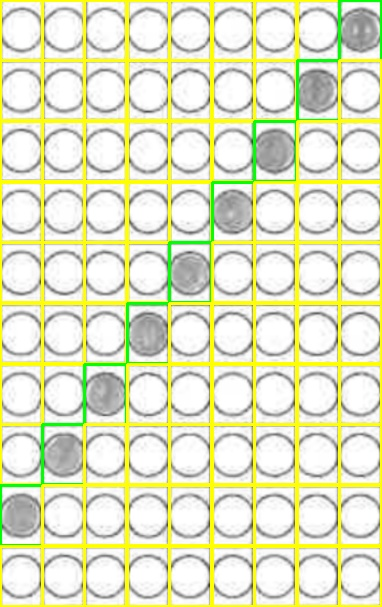
\includegraphics[width=\linewidth]{figures/result.jpg}
        \caption*{Ảnh trích xuất thông tin 1}
    \end{minipage}
    \hfill
    \begin{minipage}[b]{0.45\linewidth}
        \centering
        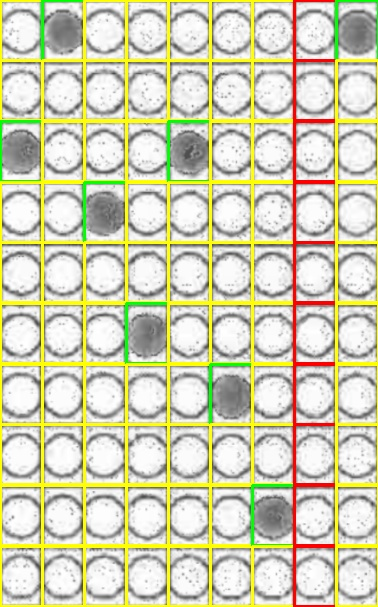
\includegraphics[width=\linewidth]{figures/result (1).jpg}
        \caption*{Ảnh trích xuất thông tin 2}
    \end{minipage}
    \caption{Kết quả trực quan hóa vùng metadata được phát hiện}
    \label{fig:result-metadata}
\end{figure}


\section{Đánh Giá Độ Tin Cậy và Tối Ưu Hiệu Suất}

Để đảm bảo kết quả nhận dạng chính xác, hệ thống kiểm tra định dạng metadata bằng cách so sánh số chữ số thu được với cấu trúc dữ liệu mong đợi. Các trường hợp sai lệch hoặc không rõ ràng sẽ được đánh dấu và lọc ra.

Bên cạnh đó, ảnh không đạt chuẩn sẽ được xử lý bằng cách điều chỉnh độ sáng, tăng tương phản và loại bỏ nhiễu, giúp cải thiện hiệu quả các bước tiếp theo.

Cuối cùng, các bước xử lý được tổ chức lại hợp lý và tối ưu tham số nội bộ, nhằm rút ngắn thời gian thực thi mà không làm giảm độ chính xác nhận dạng.

